

\documentclass[11pt,titlepage,a4paper]{report}

%INCLUSIONE PACCHETTI
%---------------------------------------------
\usepackage[italian]{babel}
\usepackage{fancyhdr}
\usepackage{graphicx}
\graphicspath{{./pics/}} % cartella di salvataggio immagini

% STILE DI PAGINA
%---------------------------------------------
\pagestyle{fancy}
\renewcommand{\sectionmark}[1]{\markright{\thesection.\ #1}}
\lhead{\nouppercase{\rightmark}}
\rhead{\nouppercase{\leftmark}}
\renewcommand{\chaptermark}[1]{%
\markboth{\thechapter.\ #1}{}}

%Ridefinisco lo stile plain della pagina
\fancypagestyle{plain}{%
	\lhead{
\includegraphics[height=50pt]{logo.eps}}
	\chead{}
	\rhead{HappyCode inc \\ happycodeinc@gmail.com}
	\lfoot{BR-jsys}
	\cfoot{\thepage}
	\renewcommand{\headrulewidth}{1pt}
	\renewcommand{\footrulewidth}{1pt}
}
% layout
\begin{document}
%definizione variabili 
\newcommand{\lv}{ 1.3 } % latest version
\newcommand{\dt}{ Manuale Utente }% Document title
\newcommand{\Grammatica}{} % paragrafo dove si trova la spiegazione della grammatica
%common variables
\newcommand{\br}{\underline{business rule}}
\newcommand{\brs}{\underline{business rules}}
\newcommand{\bo}{\underline{business object}}
\newcommand{\bos}{\underline{business objects}}
\newcommand{\rp}{\underline{repository}}
\newcommand{\brp}{BusinessRuleParser}
\newcommand{\brl}{BusinessRuleLexer}
\newcommand{\BR}{\underline{BusinessRule}}

%nomi dei componenti
\newcommand{\AT}{Alessia Trivellato}
\newcommand{\ET}{Elena Trivellato}
\newcommand{\FC}{Filippo Carraro}
\newcommand{\LA}{Luca Appon}
\newcommand{\MB}{Michele Bortolato}
\newcommand{\MT}{Marco Tessarotto}
\newcommand{\MM}{Mattia Meroi}%altre variabili
% ultime versioni dei documenti da modificare solo alla fine
\newcommand{\AR}{AnalisiDeiRequisiti.2.6.pdf}
\newcommand{\DdP}{DefinizioneDiProdotto.0.9.pdf}
\newcommand{\G}{ Glossario.1.8.pdf }
\newcommand{\NdP}{NormeDiProgetto.2.0.pdf}
\newcommand{\PdQ}{ PianoDiQualifica.2.0.pdf }
\newcommand{\PdP}{ PianoDiProgetto.1.7.pdf }
\newcommand{\ST}{SpecificaTecnica.1.5.pdf}
\newcommand{\TR}{TestReport.0.7.pdf}
\newcommand{\MU}{ManualeUtente.0.3.pdf}%nomi documenti
%fine definizione variabili
\hyphenation{
 a-na-lo-go
 as-so-cia-zio-ne
 %attività non si può inserire come tutte le parole accentate che vanno messe nel testo semplice scritte at\-ti\-vi\-tà o come variabile
 coe-ren-za
 com-po-nen-ti
 des-crit-te
 des-cri-zio-ni
 di-a-gram-ma
 di-a-gram-mi
 e-le-men-to
 e-se-gui-re
 e-si-sten-ti
 es-pli-ci-to
 glo-bal-men-te
 glos-sa-rio
 li-vel-lo
 ne-ces-sa-rio
 per-met-te-re
 re-po-si-to-ry
 re-vi-sio-na-men-to
 ri-chies-te
 se-gna-la-ta
 va-li-da-zio-ne
 va-ria-bi-li
 ve-ri-fi-ca-re
 vi-sua-liz-za-te
 e-ven-tua-li
 o-pe-ra-zio-ne
 ar-chi-via-zio-ne
 mo-di-fi-ca
}


%sillabazione
\begin{titlepage}
\begin{center}
\vspace*{0.5in}

\includegraphics{logo.eps}
\vspace*{0.2in}

{\Large \textbf{BR-jsys}}
{\Large \emph{business rules} per sistemi gestionali in architettura J2EE } 
\vspace{2in}

\Huge \textsc{ \dt }

\end{center}
\end{titlepage}
\vspace*{0.5in}%pagina del titolo

\begin{center}
\thispagestyle{plain}
\begin{table}[htbp]
\large{
\begin{tabular}{l}
\Large{\textbf{\textsf{Capitolato: ''BR-jsys``}}} \\
\begin{tabular}{|p{6cm}|p{6cm}|} \hline
\textbf{Data creazione:} & 2008/02/25 \\ \hline
\textbf{Versione:} & \lv \\ \hline
\textbf{Stato del documento:} & Formale, esterno \\ \hline
% ----------------------------------------------------------------------------autori
\textbf{Redazione:} &  \AT, \LA \\ \hline
\textbf{Revisione:} & \FC \\ \hline
\textbf{Approvazione:} & \MM \\ \hline
\end{tabular} \\
\end{tabular}
}
\end{table}

\begin{table}[hbtp]
\large{
\begin{tabular}{l}
\Large{\textbf{\textsf{Lista di distribuzione}}} \\

\begin{tabular}{|p{6cm}|p{6cm}|} \hline
{HappyCode inc}& Gruppo di lavoro\\ \hline
{Tullio Vardanega, Renato Conte}& Rappresentanti del committente \\ \hline
{Zucchetti S.r.l}& Azienda committente\\ \hline
\end{tabular} \\
\end{tabular}
}
\end{table}
\begin{table}[hbtp]

\Large{\textbf{\textsf{Diario delle modifiche}}} \\
\begin{small}
\begin{tabular}[t]{|p{1,2cm}|p{1.9cm}|p{2.9cm}|p{5cm}|} \hline
Versione & Data & Autore & Descrizione \\ \hline
%-------------------------------------------------------------------------------diario modifiche

1.3 & 08/03/2008 & \MM & Correzione documento. \\ \hline
1.2 & 07/03/2008 & \LA & Aggiunto immagini. \\ \hline
1.1 & 06/03/2008 & \AT & Correzione documento. \\ \hline
1.0 & 06/03/2008 & \AT & Aggiunta sezione ``Convenzioni usate''. \\ \hline
0.9 & 05/03/2008 & \LA & Aggiunto Sommario.\\ \hline
0.8 & 05/03/2008 & \MM & Evidenziazione dei termini contenuti nel documento \G .\\ \hline
0.7 & 04/03/2008 & \MM & Aggiunta link ipertestuali all'indice del documento.\\ \hline
0.6 & 04/03/2008 & \MT & Modifica al layout, introduzione totale pagine e autori nel diario delle modifiche.\\ \hline
0.8 & 06/03/2008 & \LA & Stesura sezione ``Requisiti minimi''.\\ \hline
0.7 & 05/03/2008 & \LA & Stesura sezione ``Caratteristiche del servizio''.\\ \hline
0.6 & 05/03/2008 & \AT & Stesura sezione ``Appendice''.\\ \hline
0.5 & 04/03/2008 & \AT & Inserimento e stesura sezione ``Descrizione della grammatica''.\\ \hline
0.4 & 03/04/2008 & \LA & Inserimento immagine 3.1, 3.2, 3.2.2, 3.3, 3.4.\\ \hline
0.3 & 02/03/2008 & \AT & Stesura sezione ``Azioni richieste/permesse''.\\ \hline
0.2 & 01/03/2008 & \AT & Completamento paragrafo ``Istruzioni per l'uso''.\\ \hline
0.1 & 25/02/2008 & \AT & Stesura preliminare del documento.\\ \hline

\end{tabular} \\
\end{small}

\end{table}
\end{center}
\newpage

\tableofcontents 
\chapter*{Sommario}
\addcontentsline{toc}{chapter}{I Sommario}
Il presente documento contiene la descrizione d'uso del sistema \underline{BR-jsys}, con raffinamento della descrizione delle singole operazioni eseguibili su tale sistema. Per un corretto funzionamento del prodotto invitiamo l'utente a seguire le specifiche di questo documento.

\chapter*{Glossario}
\addcontentsline{toc}{chapter}{II Glossario}
Viene fornito come documento esterno chiamato \G. 
\subsection{Convenzioni usate}
Per permetterne una facile individuazione, i termini contenuti nel ``\G'' sono sottolineati nei vari documenti da noi consegnati.

\chapter{Introduzione}
Il presente documento contiene la definizione dell'architettura logica del sistema ``\textbf{\underline{BR-jsys}}'', con una descrizione pi\`u accurata di ogni singola componente.
\section{Definizione dell'utente del prodotto}
Il prodotto \`e rivolto ad un utente al quale non sono richieste particolari conoscenze nel campo informatico. A tale scopo il software mette a dispozione:
\begin{itemize}
\item un'interfaccia grafica user-friendly;
\item messaggi di testo che aiutano l'utente dando informazione aggiuntive sullo stato del prodotto ``\underline{BR-jsys}''.
\end{itemize}
\section{Come leggere il manuale}
Questo manuale presenta il sistema ``\underline{BR-jsys}'' da noi realizzato e insegna come usare tutte le funzioni ad esso correlate. \`E organizzato in tre sezioni, in modo da rendere facile il reperimento delle informazioni desiderate:
\begin{itemize}
\item \underline{SEZIONE GENERALE:} dedicata alla descrizione generale del prodotto. Fornisce informazioni di base sul funzionamento del prodotto.
\item \underline{SEZIONE DETTAGLIATA:} dedicata alla descrizione dettagliata. Indispensabile per un corretto utilizzo di ogni singola parte del prodotto.
\item \underline{SEZIONE APPENDICE:} riporta gli errori pi\`u comuni che l'utente pu\`o riscontrare durante l'utilizzo del prodotto e il glossario per chiarire la terminologia da noi adottata.
\end{itemize}
Verranno riportati quindi tutti i passi che si possono effettuare, grazie anche all'ausilio di immagini dell'applicazione.
\section{Documenti utili}
Il presente manuale descrive totalmente il sistema e non richiede la lettura di ulteriori documenti. Tuttavia ogni utente deve avere installato nel proprio pc ``\textbf{eXist}'' in quanto vero e proprio requisito di sistema. 
\section{Come riportare problemi e malfunzionamenti}
Il prodotto software \`e dotato di un sistema di archiviazione svn. Tale archivio fornisce una sezione ``issues'' all'URL: \\ 
\textbf{``http://code.google.com/p/br-jsys/issues/list''}, che visualizza in qualsiasi momento la lista aggiornata di tutti i problemi e malfunzionamenti da noi riscontrati. Attraverso questo sistema ogni componente del gruppo potr\`a creare un ``new issue'', assegnandogli una priorit\`a che varier\`a a seconda della gravit\`a del problema. Ogni issue conterr\`a inoltre il nome dell'utente che lo ha aggiunto nella lista, oltre ad uno status (new, accepted, started, verified, etc...) che in qualsiasi momento ogni membro del gruppo potr\`a aggiornare. 

\chapter{Descrizione generale}
Il prodotto ``\underline{BR-jsys}'' permette di testare la consistenza di business objects. A tale scopo il software mette a disposizione, attraverso la propria interfaccia grafica, la possibilit\`a di inserimento di \underline{business rules} validate, cancellazione e querying nel \rp.
\section{Descrizione del linguaggio}
In questa sezione faremo una descrizione dettagliata della grammatica da noi generata per rappresentare le \underline{business rules}. 
\subsection{Struttura \underline{business rule}}
Una \underline{business rule} pu\`o essere formata da:
\begin{itemize}
\item una \textbf{regola} atomica;
\item un insieme di \textbf{regole} collegate tra loro attraverso operatori booleani (AND \textbar OR).
\end{itemize}
\subsection{Struttura regola}
Ogni singola regola \`e formata da \textbf{espressioni} collegate tra loro attaverso operatori di confronto (= \textbar\ != \textbar\ \textless\ \textbar\ \textgreater\ \textbar\ \textless= \textbar\ \textgreater=). Alla regola pu\`o venire associato un ``\textbf{message}'' (opzionale), col compito di fornire informazioni aggiuntive sullo stato di validazione della \underline{business rule}. In particolare, il testo di tale messaggio verr\`a visualizzato quando si cerca di validare un business object che non rispetta una o pi\`u regole presenti nel \rp.
\subsection{Struttura espressione}
Un'espressione \`e formata da campi dati che posso essere di 3 tipi:
\begin{itemize}
\item Float;
\item Bool;
\item String. 
\end{itemize}
\textbf{Float} permette operazioni di:
\begin{itemize}
\item[-] addizione;
\item[-] sottrazione;
\item[-] moltiplicazione;
\item[-] divisione.
\end{itemize}
Queste possono essere accompagnate da funzioni quali:
\begin{itemize}
\item[-] AVG (media aritmetica);
\item[-] COUNT (contatore);
\item[-] SUM (somma). 
\end{itemize}
\textbf{Bool} permette operazioni quali:
\begin{itemize}
\item[-] \&\& (congiunzione logica);
\item[-] \textbar\textbar\ (disgiunzione logica).
\end{itemize}
oltre alla funzione:
\begin{itemize}
\item[-] NOT (negazione logica). 
\end{itemize}
\textbf{String} permette invece solo operazioni di confronto.
\subsection{Struttura message}
Un message pu\`o essere formato da:
\begin{itemize}
\item lettere maiuscole (A-Z);
\item lettere minuscole (a-z);
\item numeri (0-9);
\item spazi vuoti;
\item i seguenti caratteri di punteggiatura: '.'  '?'  '!'  '\_'  '-'  '\~'
\item i seguenti caratteri speciali \^ e \~ \\
\end{itemize}
\subsection{Esempi di \underline{business rules}}
Faremo ora, per una maggiore comprensione del linguaggio, alcuni esempi di \underline{business rules}.
\begin{itemize}
\item \textbf{ESEMPIO 1} \\
\underline{REGOLA NEL LINGUAGGIO NATURALE:} \\
L'azienda deve essere la IBM. La somma delle entrate deve essere maggiore di quella delle uscite altrimenti deve ritornare un messaggio con scritto ``errore nei calcoli''. \\
\underline{REGOLA NEL LINGUAGGIO CREATO:} \\
azienda=``IBM'' AND SUM(entrate)\textgreater\ SUM(uscite) message(``errore nei calcoli'')
\item \textbf{ESEMPI0 2} \\
\underline{REGOLA NEL LINGUAGGIO NATURALE:} \\
Il nome dello studente deve essere Lisa. I suoi crediti devono essere almeno 180 altrimenti deve ritornare un messaggio con scritto ``totale crediti sbagliato''. I suoi anni di corso devono essere non pi\`u di tre altrimenti torna un messaggio con scritto ``risulti fuori corso''.  \\
\underline{REGOLA NEL LINGUAGGIO CREATO:} \\
nome=``Lisa'' AND SUM(crediti)\textgreater =180 message(``totale crediti sbagliato'') AND COUNT(anni)\textless =3 message(``risulti fuori corso'')
\end{itemize}
\subsection{Rappresentazione in XML}
Mostriamo ora come vengono rappresentati i vari simboli e operatori della grammatica nella loro rappresentazione in XML.
\begin{table}[htbp]
\begin{tabular}{||p{3cm}||p{6.5cm}||}
\hline
\textbf{REGOLA:} & \textbf{XML:} \\ \hline
& \\ \hline
X=Y & \textless Conf type=``=''\textgreater \\
&   X \\
&   Y \\ 
& \textless /Conf\textgreater \\ \hline
X!=Y & \textless Conf type=``!=''\textgreater \\
&  X \\
&  Y \\ 
& \textless /Conf\textgreater\\ \hline
X\textless Y & \textless Conf type=``\&lt''\textgreater \\
&  X \\
&  Y \\ 
& \textless /Conf\textgreater\\ \hline
X\textgreater Y & \textless Conf type=``\&gt''\textgreater \\
&  X \\http://mail.google.com/mail/
&  Y \\ 
& \textless /Conf\textgreater\\ \hline
X\textless=Y & \textless Conf type=``\&lt=''\textgreater \\
&  X \\
&  Y \\ 
& \textless /Conf\textgreater\\ \hline
X\textgreater =Y &  \textless Conf type=``\&gt=''\textgreater \\
&  X \\
&  Y \\ 
& \textless /Conf\textgreater\\ \hline
& \\ \hline
\end{tabular} \\
\end{table}

\begin{table}[htbp]
\begin{tabular}{||p{3cm}||p{6.5cm}||}
\hline
X AND Y & \textless ORule type=``AND''\textgreater \\
&  X \\
&  Y \\
& \textless /OpRule\textgreater \\ \hline
X OR Y & \textless ORule type=``OR''\textgreater \\
&  X \\
&  Y \\
& \textless /OpRule\textgreater \\ \hline
& \\ \hline
SUM(X) & \textless Fun type=``SUM''\textgreater\\ 
&  X \\
& \textless /Fun\textgreater \\ \hline
COUNT(X) & \textless Fun type=``COUNT''\textgreater\\ 
&  X \\
& \textless /Fun\textgreater \\ \hline
AVG(X) & \textless Fun type=``AVG''\textgreater\\ 
&  X \\
& \textless /Fun\textgreater \\ \hline
& \\ \hline
X+Y & \textless OFloat type=``+''\textgreater\\
&  X \\
&  Y \\
& \textless /OFloat\textgreater \\ \hline
X-Y & \textless OFloat type=``-''\textgreater\\
&  X \\
&  Y \\
& \textless /OFloat\textgreater \\ \hline
X*Y & \textless OFloat type=``*''\textgreater\\
&  X \\
&  Y \\
& \textless /OFloat\textgreater \\ \hline
X/Y & \textless OFloat type=``/''\textgreater\\
&  X \\
&  Y \\
& \textless /OFloat\textgreater \\ \hline
& \\ \hline
X \textbar\textbar Y & \textless OBool type=``\textbar\textbar''\textgreater\\
&  X \\
&  Y \\
& \textless /OBool\textgreater \\ \hline
X \&\& Y & \textless OBool type=``\&amp;\&amp;''\textgreater \\
&  X \\
&  Y \\
& \textless /OBool\textgreater \\ \hline
\end{tabular} \\
\end{table}

\begin{table}[htbp]
\begin{tabular}{||p{3cm}||p{6.5cm}||}
\hline
NOT(X) & \textless BoFun type=``NOT''\textgreater \\
&  Y \\
& \textless /BoFun\textgreater \\ \hline
& \\ \hline 
4.0 & \textless FLOAT \textgreater4.0\textless /FLOAT\textgreater \\ \hline
true & \textless BOOL \textgreater true\textless /BOOL\textgreater \\ \hline
``stringa'' & \textless STRING \textgreater ``stringa'' \textless /STRING\textgreater \\ \hline
`campo dati' &\textless FIELD \textgreater campo dati \textless /FIELD\textgreater \\ \hline
\end{tabular} \\
\end{table}

\section{Caratteristiche del servizio}
Una volta avviato, il sistema ``\underline{BR-jsys}'' offre all'utente:
\begin{itemize}
\item[-] un'elevata configurabilit\`a ed estendibilit\`a dei business objects;
\item[-] un linguaggio per la definizione di \underline{business rules};
\item[-] un validatore che consenta l'accettazione di nuove \underline{business rules}, soltanto se esse sono scritte secondo le specifiche del linguaggio creato;
\item[-] un repository per immagazzinare le \underline{business rules};
\item[-] una competa gestione del repository tramite interfacciamento ad ``eXist'';

\item[-] un aiuto agli utenti meno esperti attraverso  messaggi di errore;
\item[-] una semplice interfaccia per operare su questo sistema.
\end{itemize}
\section{Requisiti minimi}
\subsection{Requisiti sofware}
\begin{itemize}
\item \underline{Sistema operativo:}
\begin{itemize}
\item[-] Linux: tutte le piattaforme con qualsiasi distribuzione.
\item[-] Windows: Windows2000 e WindowsXp home/professional.
\item[-] MacOSX: 10.4.
\end{itemize}
\item \underline{eXist} 1.2;
\item \underline{Java Runtime Environment (JRE)} 1.6.
\end{itemize}
Per usufruire del servizio \`e quindi necessario possedere una connessione con il DBMS ``eXist''.
\subsection{Requisiti hardware}
Per un corretto e scorrevole funzionamento del software sono richiesti:
\begin{itemize}
\item Processore 850Mhz.
\item 128Mb Ram.
\end{itemize}

\chapter{Istruzioni per l'uso}
\section{Descrizione funzionale}
Di seguito \`e riportata la descrizione delle funzioni del prodotto. Ad ogni passo \`e stata associata una figura, in modo da daterminare senza amibiguit\`a il contesto dell'applicazione.
\subsection{Installazione}
Per utilizzare il prodotto \`e necessario che questo sia installato sulla macchina server. La sua architettura prevede che venga usato ``eXist'', scaricabile liberamente al sito \textbf{http://exist.sourceforge.net}. Dopodich\`e da macchina:
\begin{itemize}
\item \underline{Linux o MacOSX:} 
\begin{itemize}
\item[-] avviare il prompt dei comandi (\textbf{shell});
\item[-] accedere alla cartella ``\textbf{BR-jsys}'' fornita; 
\item[-] digitare il comando ``\textbf{sh install}''.
\end{itemize}
% mettere una foto di come avviene l'installazione in linux
\item \underline{Windows:}
\begin{itemize} 
\item[-] avviare il prompt dei comandi (\textbf{shell});
\item[-] accedere alla cartella ``\textbf{BR-jsys}'' fornita;
\item[-] cliccare su ``\textbf{install.exe}''.
\end{itemize}
% mettere una foto di come avviene l'installazione in Windows
\end{itemize}
L'installazione si preoccuer\`a di sistemare le dipendenze per il corretto funzionamento del programma.
\subsection{Avvio dell'applicazione}
Per avviare il programma, una volta terminata l' installazione, sia in Linux che in Windows che in MacOSX occorre:
\begin{itemize}
\item[-] avviare il prompt dei comandi (\textbf{shell});
\item[-] accedere alla cartella ``\textbf{\underline{BR-jsys}}'' fornita; 
\item[-] digitare ``\textbf{BR-jsys.start}''.
\end{itemize}
% mostrare una foto con i passi per avviare l'applicazione
 Dopo un breve periodo di caricamento apparir\`a la schermata di login (figura 3.0), nella quale l'utente che accede per la prima volta al servizio dovr\`a digitare i seguenti dati: 
\begin{itemize}
\item username
\item password
\end{itemize}
\begin{center}
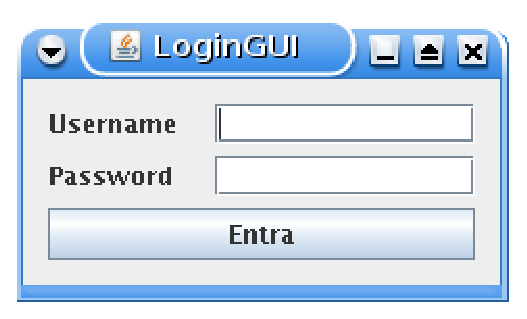
\includegraphics[width=0.4\textwidth]{manuale_utente/login.eps}\\
 figura 3.0: schermata di login
\end{center}
I dati di autenticazione immessi sono quelli utilizzati per la registrazione al server ``\underline{eXist}''. Tutti i dati richiesti dovranno essere insieriti prestando attenzione alla scelta della password, la quale dovr\`a avere una complessit\`a elevata. 
\subsubsection{Esiti}
Nel caso di login eseguita correttamente, verr\`a lanciata la schermata principale (figura 3.1).
Altrimenti viene mostrato un messaggio d'errore:
\begin{itemize}
\item Errore server eXsit spento (figura 3.0.1)
\item Errore di autenticazione (figura 3.0.2)
\end{itemize}

\begin{center}
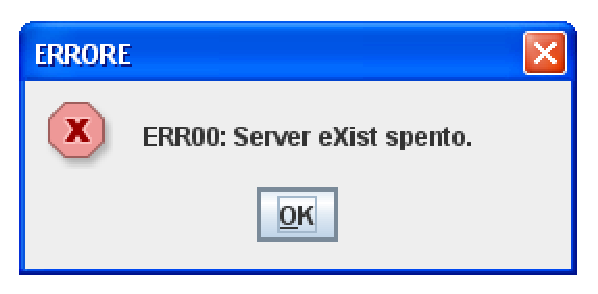
\includegraphics[width=0.5\textwidth]{manuale_utente/errore_server_spento.eps}\\
 figura 3.0.1: esempio di server spento
\end{center} 

\begin{center}
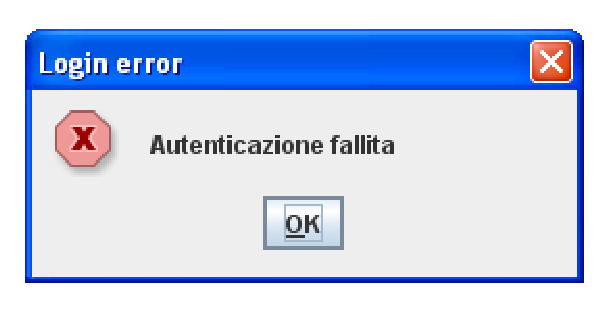
\includegraphics[width=0.5\textwidth]{manuale_utente/autenticazione_fallita.eps}\\
figura 3.0.2: esempio di username e/o password errati
\end{center} 

\section{Azioni richieste/permesse}
\begin{center}
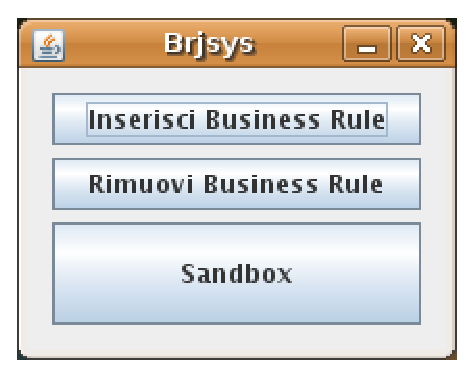
\includegraphics[width=0.4\textwidth]{manuale_utente/schermata_principale.eps}\\
 figura 3.1: schermata principale
\end{center}
A questo punto verr\`a visualizzata la schermata principale (figura 3.1).
Nella figura 3.1 vediamo illustrate le tre funzionalit\`a associate ai rispettivi bottoni:
\begin{itemize}
\item Inserisci \underline{business rule};
\item Rimuovi \underline{business rule};
\item Sandbox.
\end{itemize}
L'analisi dettagliata delle singole azioni verr\`a trattata nelle sottosezioni seguenti.
\subsection{Inserisci \underline{business rule}}
\begin{center}
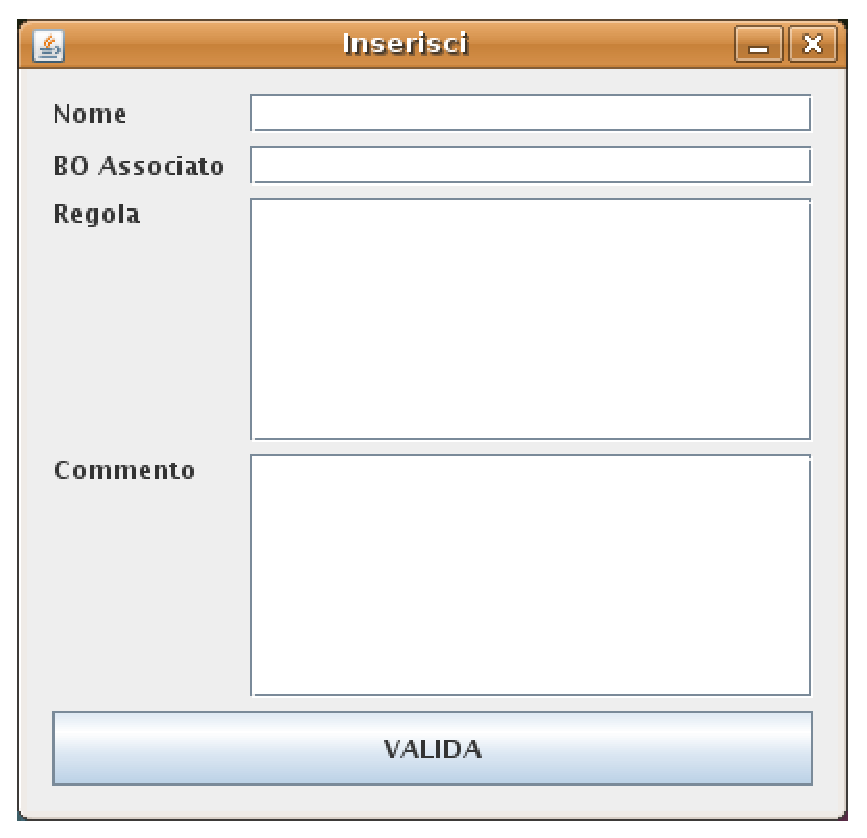
\includegraphics[width=0.7\textwidth]{manuale_utente/schermata_inserimento.eps}\\
 figura 3.2: schermata di inserimento
\end{center}
Nella figura 3.2 vediamo illustrata la schermata di inserimento di una nuova \underline{business rule}. L'utente dovr\`a inserire negli appositi spazi i campi dati richiesti:
\begin{itemize}
\item \underline{Nome:} \\
Il nome della \underline{business rule} che l'utente intende inserire (il nome dovr\`a essere significativo);
\item \underline{BO Associato:} \\
Il nome della classe del business object alla quale si vuole associare la regola;
\item \underline{Regola:} \\
 La regola scritta secondo la grammatica spiegata nel paragrafo \Grammatica;
\item \underline{Commento:} \\
Descrizione sintetica del comportamento della regola. 
\end{itemize}
L'utente dovr\`a ora cliccare sul pulsante ``\textbf{Valida}''. Se l'inserimento viene effettuato con successo verr\`a visualizzato un messaggio che ne conferma l'esito positivo, in caso contrario uno negativo. 
\begin{center}
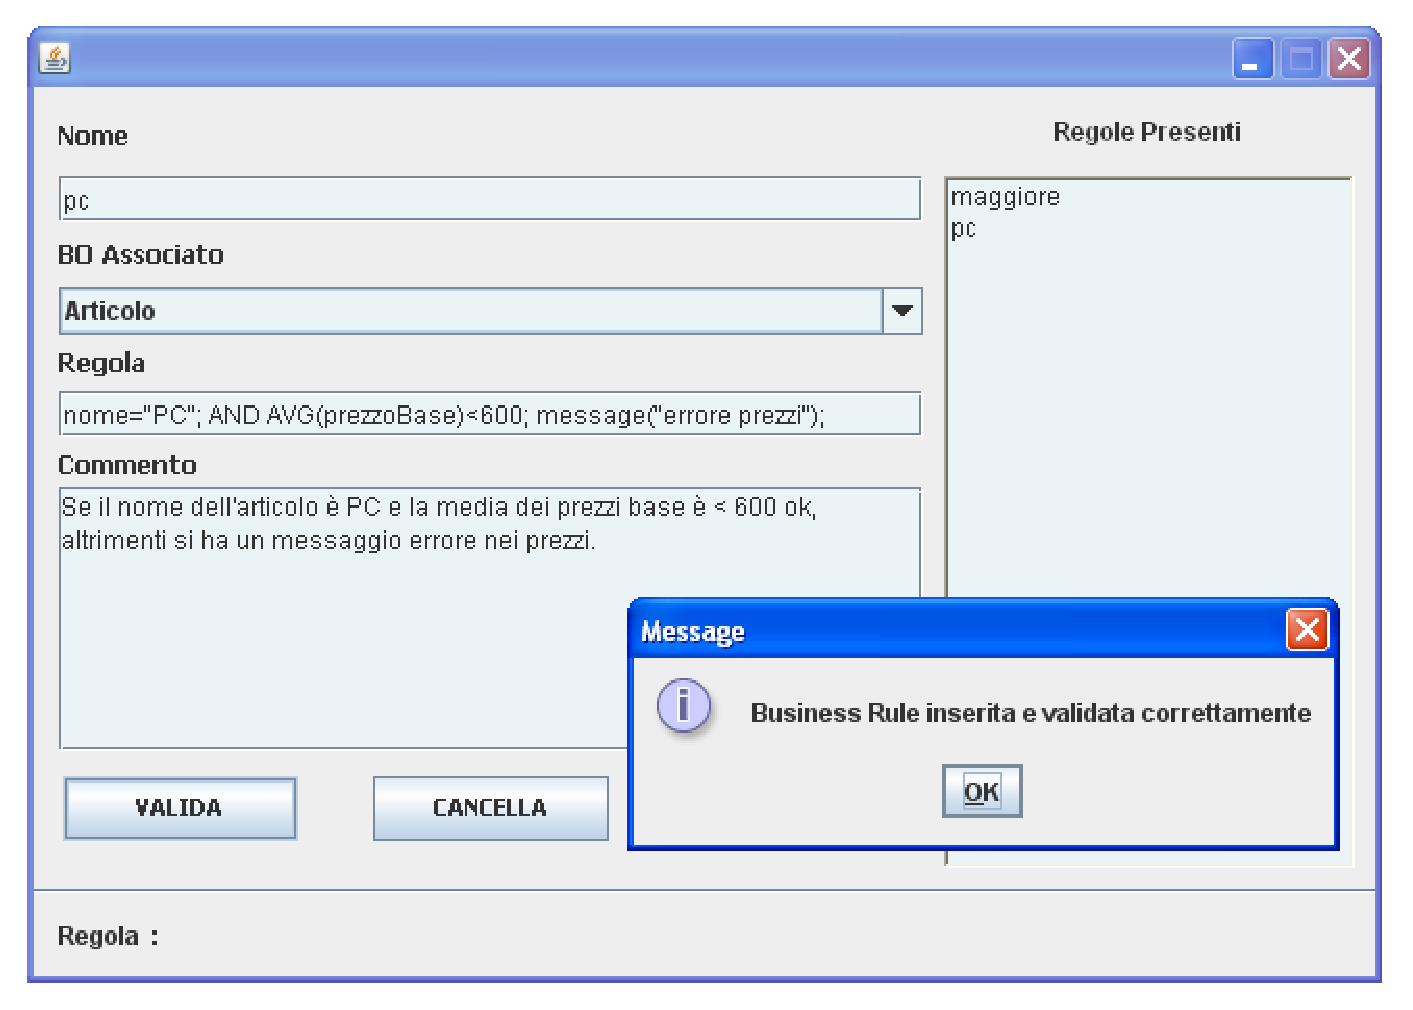
\includegraphics[width=0.7\textwidth]{manuale_utente/schermata_esempio_inserimento.eps}\\
 figura 3.2.2: esempio di inserimento
\end{center} 
\subsubsection{Esiti}
\begin{center}
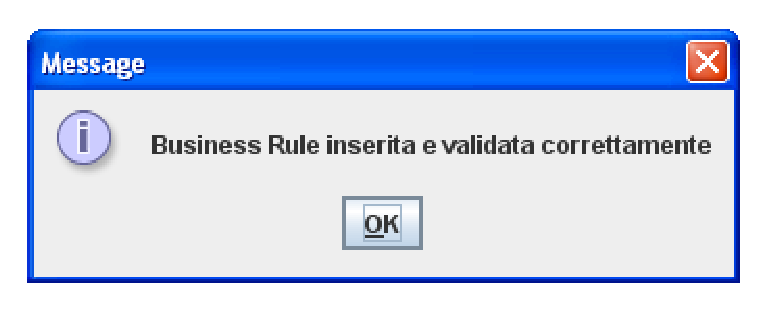
\includegraphics[width=0.7\textwidth]{manuale_utente/br_inserita.eps}\\
 figura 3.2.3: esempio inserimento effettuato
\end{center} 
La figura 3.2.3 mostra l'esito di un corretto inserimento di \underline{business rules}. La \underline{business rule} \`e stata cos\`i validata e inserita nel repository.

\begin{center}
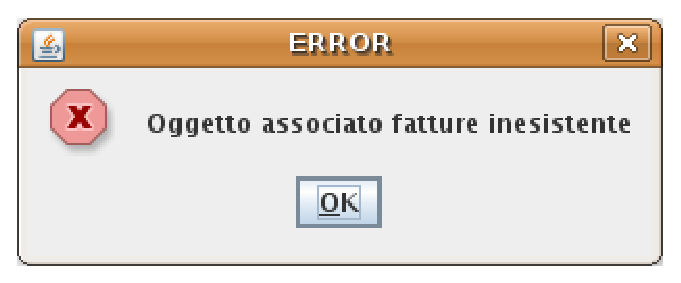
\includegraphics[width=0.5\textwidth]{manuale_utente/errore_bo_inesistente.eps}\\
 figura 3.2.4: esempio di bo associato non trovato
\end{center} 
La figura 3.2.4 mostra l'esito di un errato inserimento di \underline{business rules}. La \underline{business rule} non pu\`o essere validata e inserita nel repository in quanto il business object associato (in questo esempio ``fatture'') non \`e presente nel repository.

\begin{center}
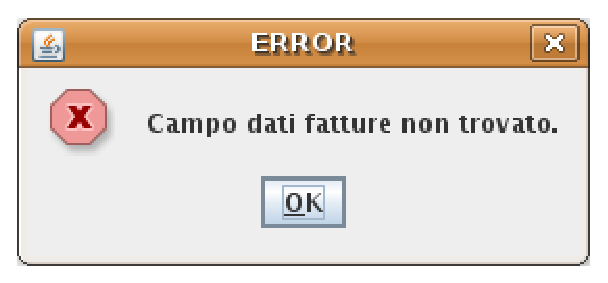
\includegraphics[width=0.5\textwidth]{manuale_utente/errore_bo_non_trovato.eps}\\
 figura 3.2.5: esempio di bo non trovato
\end{center} 
La figura 3.2.5 mostra l'esito di un errato inserimento di \underline{business rules}. La \underline{business rule} non pu\`o essere validata e inserita nel repository in quanto il business object immesso non \`e presente nel repository.

\begin{center}
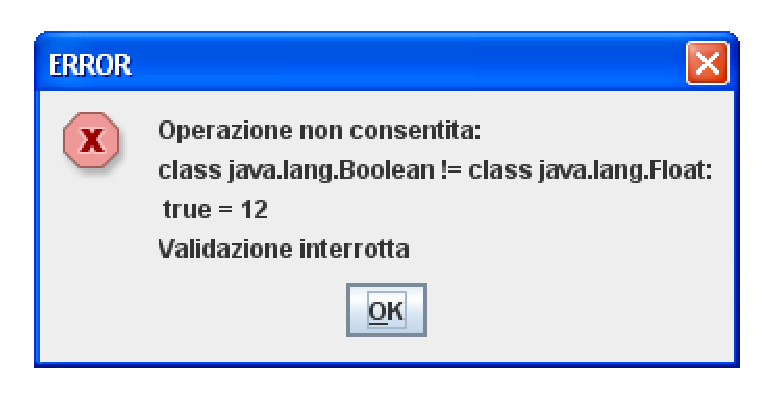
\includegraphics[width=0.7\textwidth]{manuale_utente/errore_op_non_consentita.eps}\\
 figura 3.2.6: esempio di br sintatticamente errata 
\end{center} 
La figura 3.2.6 mostra l'esito di un errato inserimento di \underline{business rules}. La \underline{business rule} non pu\`o essere validata e inserita nel repository in quanto la regola immessa (in questo caso true=12) non \`e consentita.
\\
\\
\begin{center}
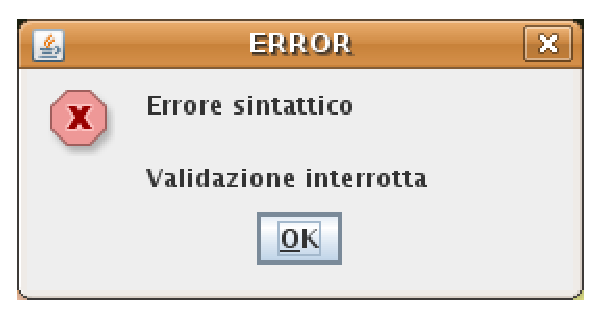
\includegraphics[width=0.5\textwidth]{manuale_utente/errore_sintattico.eps}\\
 figura 3.2.7: esempio di br errata
\end{center} 
La figura 3.2.7 mostra l'esito di un errato inserimento di \underline{business rules}. La \underline{business rule} non pu\`o essere validata e inserita nel repository in quanto la regola immessa \`e scritta in maniera errata.

\begin{center}
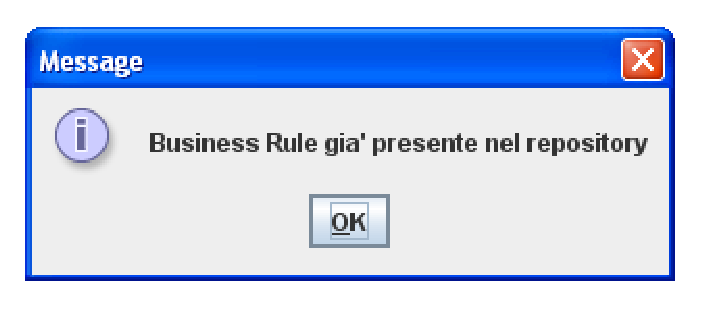
\includegraphics[width=0.6\textwidth]{manuale_utente/errore_br_gia_presente.eps}\\
 figura 3.2.8: esempio di br gi\`a inserita
\end{center} 
La figura 3.2.8 mostra l'esito di un errato inserimento di \underline{business rules}. La \underline{business rule} non pu\`o essere validata e inserita nel repository in quanto vi \`e gi\`a un'occorrenza di questa nel repository.


\subsection{Rimuovi \underline{business rule}}
\begin{center}
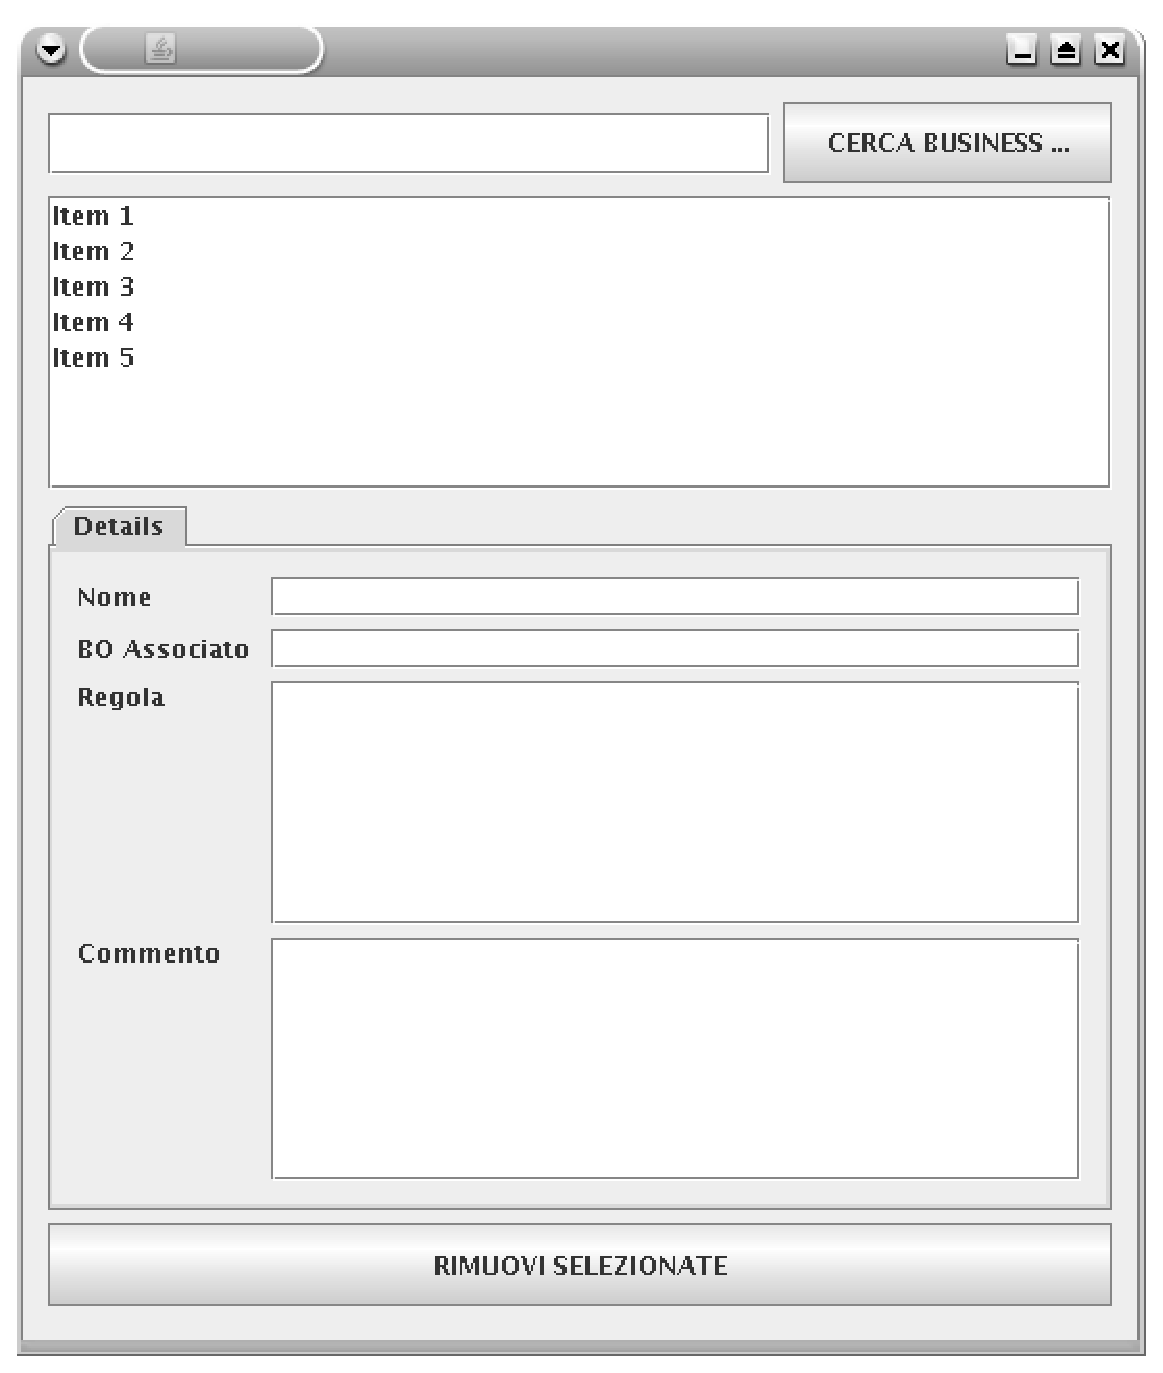
\includegraphics[width=0.7\textwidth]{manuale_utente/schermata_rimozione.eps}\\
 figura 3.3: schermata di rimozione
\end{center}
Nella figura 3.3 vediamo illustrata la schermata di cancellazione di una \underline{business rule}.
\begin{itemize}
\item Per procedere all'eliminazione l'utente avr\`a 2 modi:
\begin{enumerate}
\item inserire nell'appostito campo (TextBox) il nome della \underline{business rule} che intende rimuovere e cliccare sul pulsante ``\textbf{Cerca}''.
\item selezionare una o pi\`u \underline{business rule} dalla lista sottostante.
\end{enumerate}

\item Se la \underline{business rule} risulta presente nel repository (figura 3.3.1), comparir\`a  nel campo ``Details'' i suoi dettagli (Nome, BO Associato, Regola, Commento) figura 3.3.2. 

\begin{center}
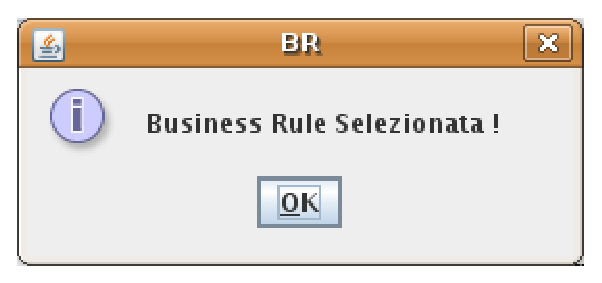
\includegraphics[width=0.5\textwidth]{manuale_utente/br_selezionata.eps}\\
 figura 3.3.1: messaggio di br trovata
\end{center} 

\begin{center}
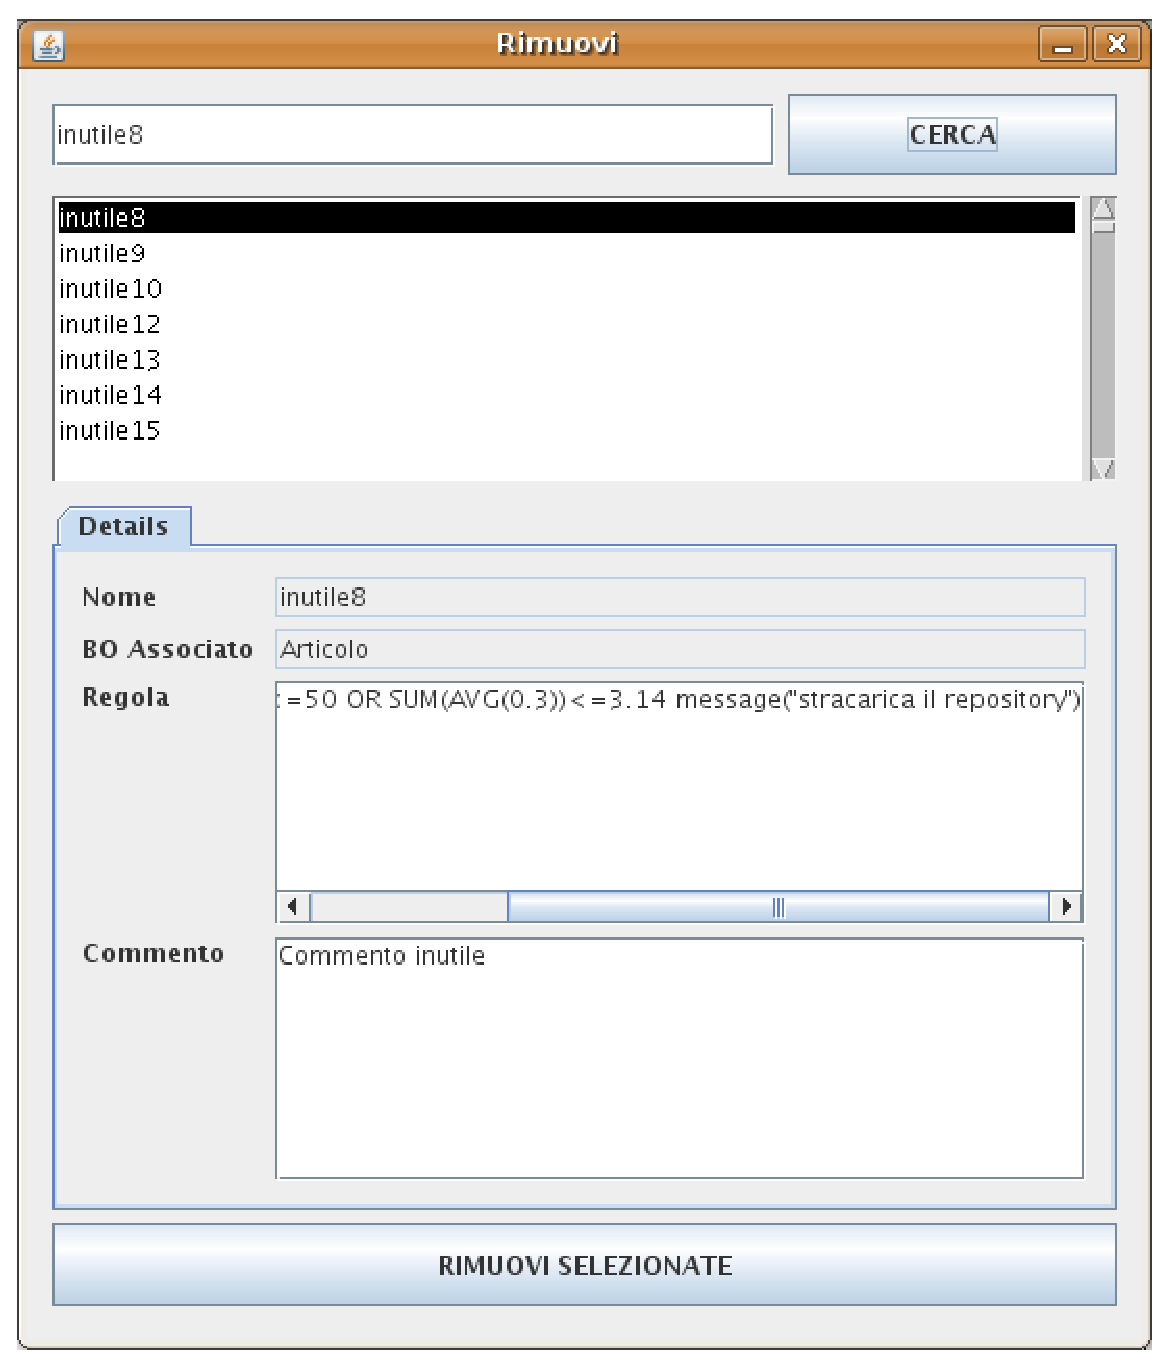
\includegraphics[width=0.7\textwidth]{manuale_utente/rimozione_br_trovata.eps}\\
 figura 3.3.2: esempio di br selezionata
\end{center} 

\begin{center}
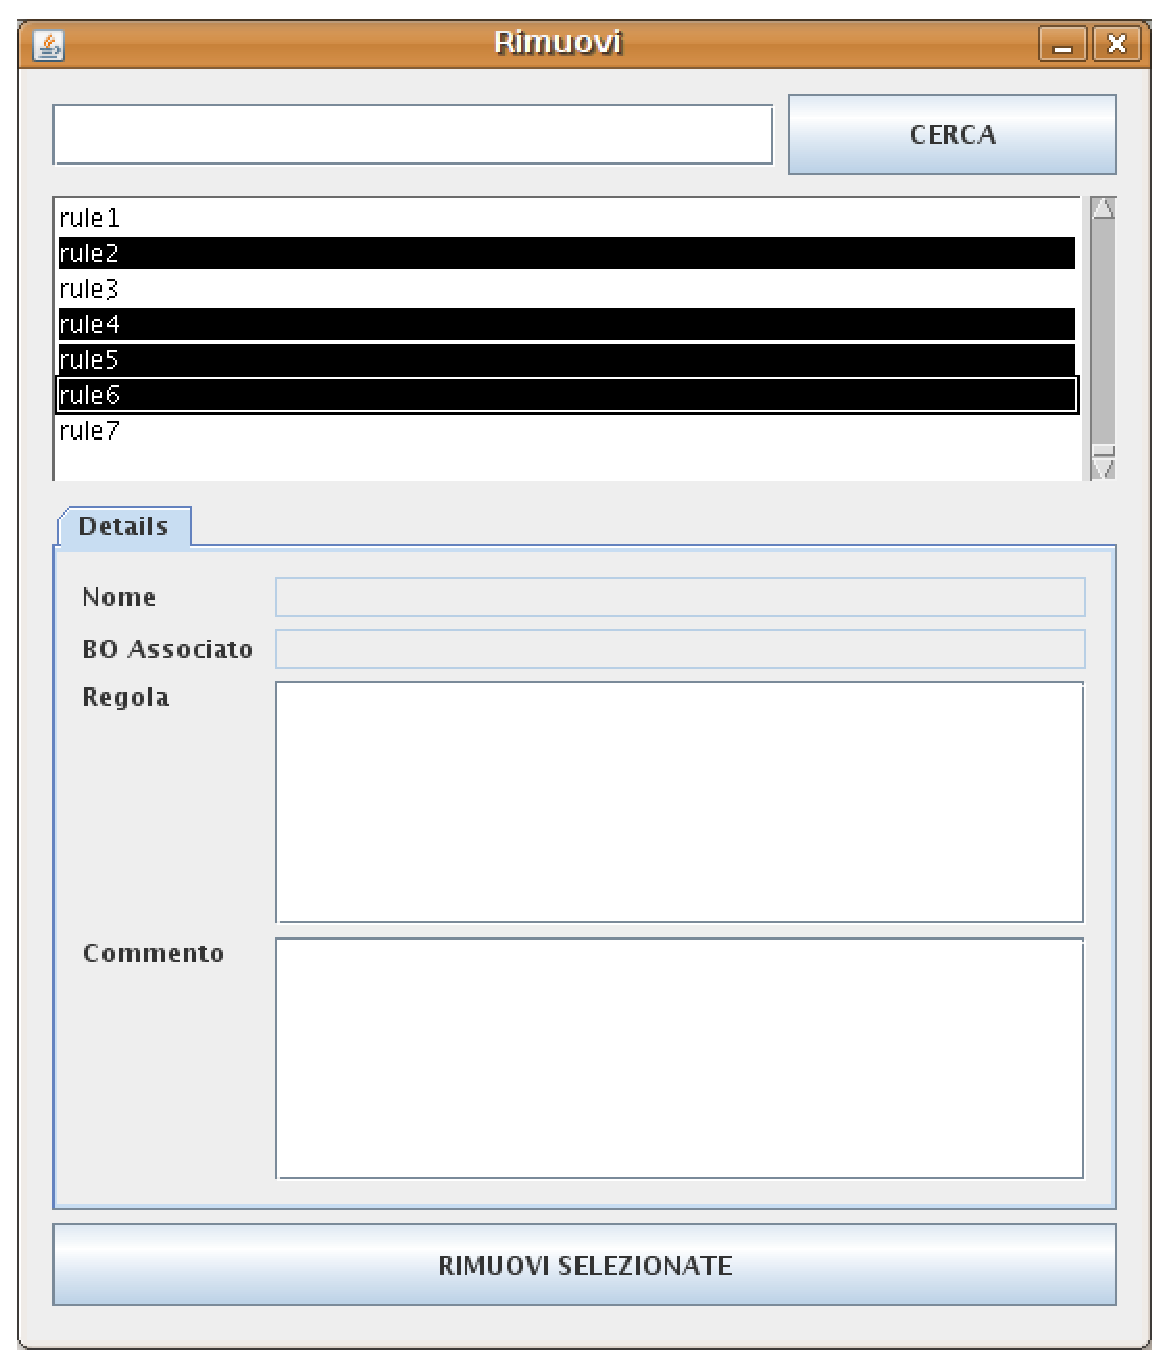
\includegraphics[width=0.7\textwidth]{manuale_utente/selezione_multipla.eps}\\
 figura 3.3.3: esempio di selezione multipla
\end{center} 

\item A questo punto baster\`a cliccare sul pulsante ``\textbf{Rimuovi Selezionate}'' e dare conferma di rimozione figura 3.3.4.  
\end{itemize}

\begin{center}
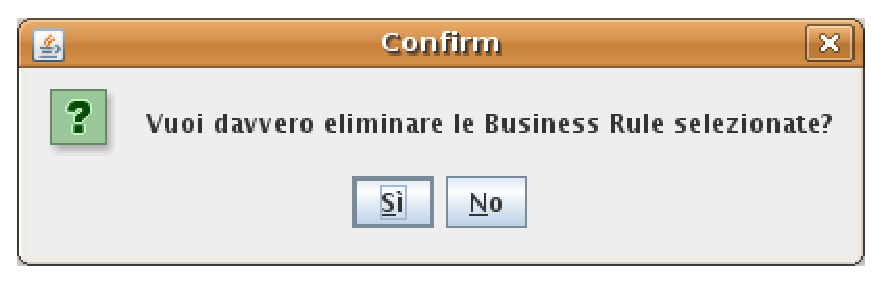
\includegraphics[width=0.7\textwidth]{manuale_utente/conferma_rimozione.eps}\\
 figura 3.3.4 messaggio di conferma
\end{center} 

Se la cancellazione viene effettuata con successo verr\`a visualizzato un messaggio che ne conferma l'esito positivo, in caso contrario uno negativo.
\subsubsection{Esiti}
 
\begin{center}
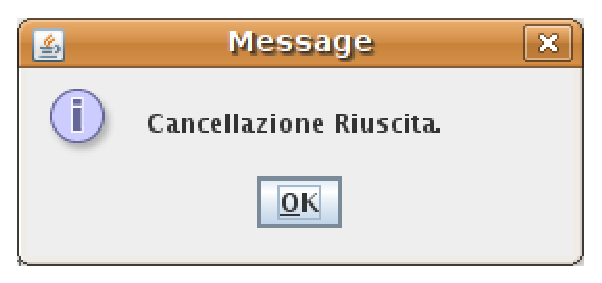
\includegraphics[width=0.5\textwidth]{manuale_utente/cancellazione_riuscita.eps}\\
figura 3.3.5 messaggio di br rimossa
\end{center} 
La figura 3.3.5 mostra la conferma di rimozione di \underline{business rules}. La \underline{business rule} \`e stata trovata dal repository.

\begin{center}
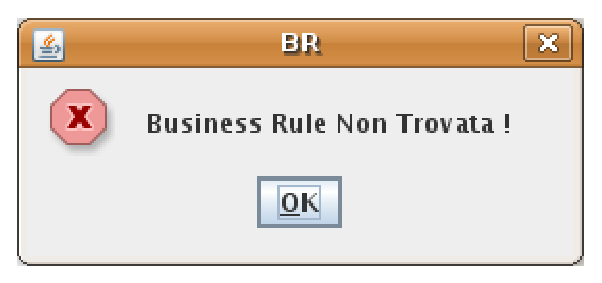
\includegraphics[width=0.5\textwidth]{manuale_utente/br_non_trovata.eps}\\
 figura 3.3.6 messaggio di br non trovata
\end{center} 
La figura 3.3.6 mostra l'esito di un'errata rimozione di \underline{business rules}. La \underline{business rule} non pu\`o essere rimossa dal repository in quanto non \`e stata trovata al suo interno.

% occorre inserire il messaggio dei due esiti
\subsection{Sandbox}
\begin{center}
 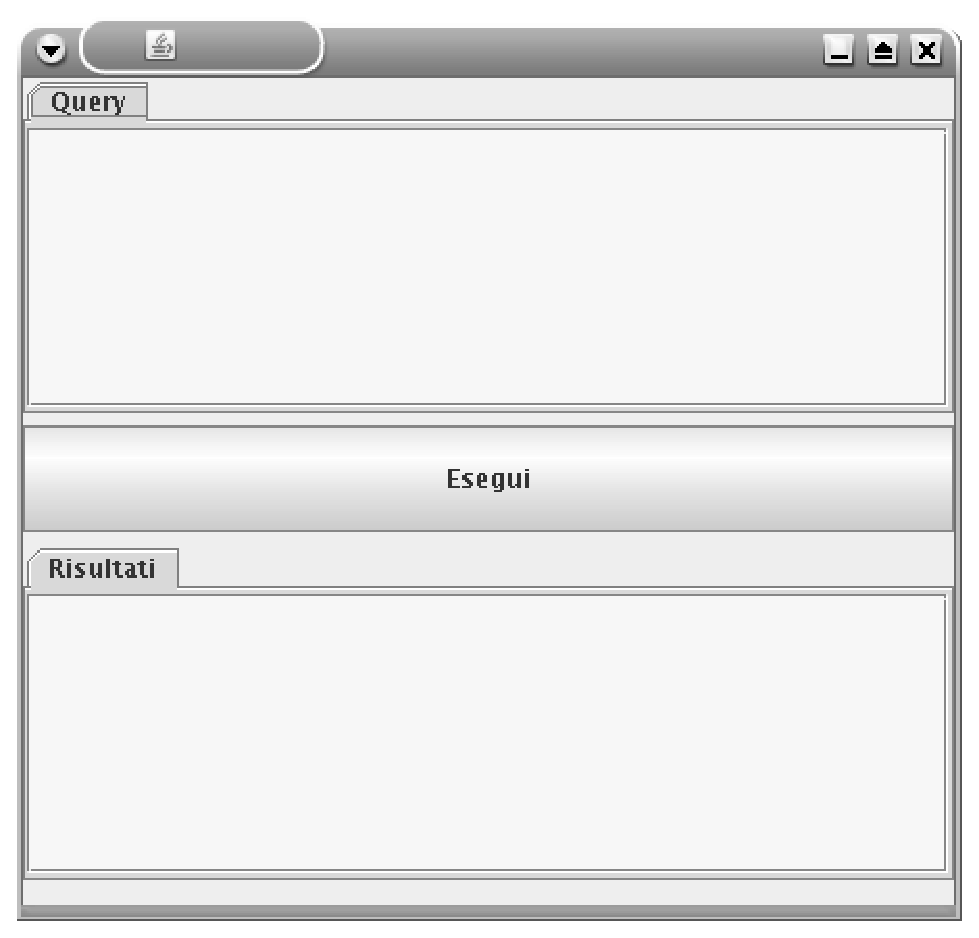
\includegraphics[width=0.7\textwidth]{manuale_utente/schermata_sandbox.eps} \\
 figura 3.4: schermata sandbox
\end{center}
Nella figura 3.4 vediamo illustrata la schermata di sandbox. Per procedere con l'interrogazione del database, l'utente dovr\`a:
\begin{itemize}
\item inserire la query (scritta in linguaggio Xquery) nell'appostito campo dati ``Query'';
\item cliccare sul pulsante ``\textbf{Esegui}''.
\end{itemize}

\subsubsection{Esiti}
\begin{center}
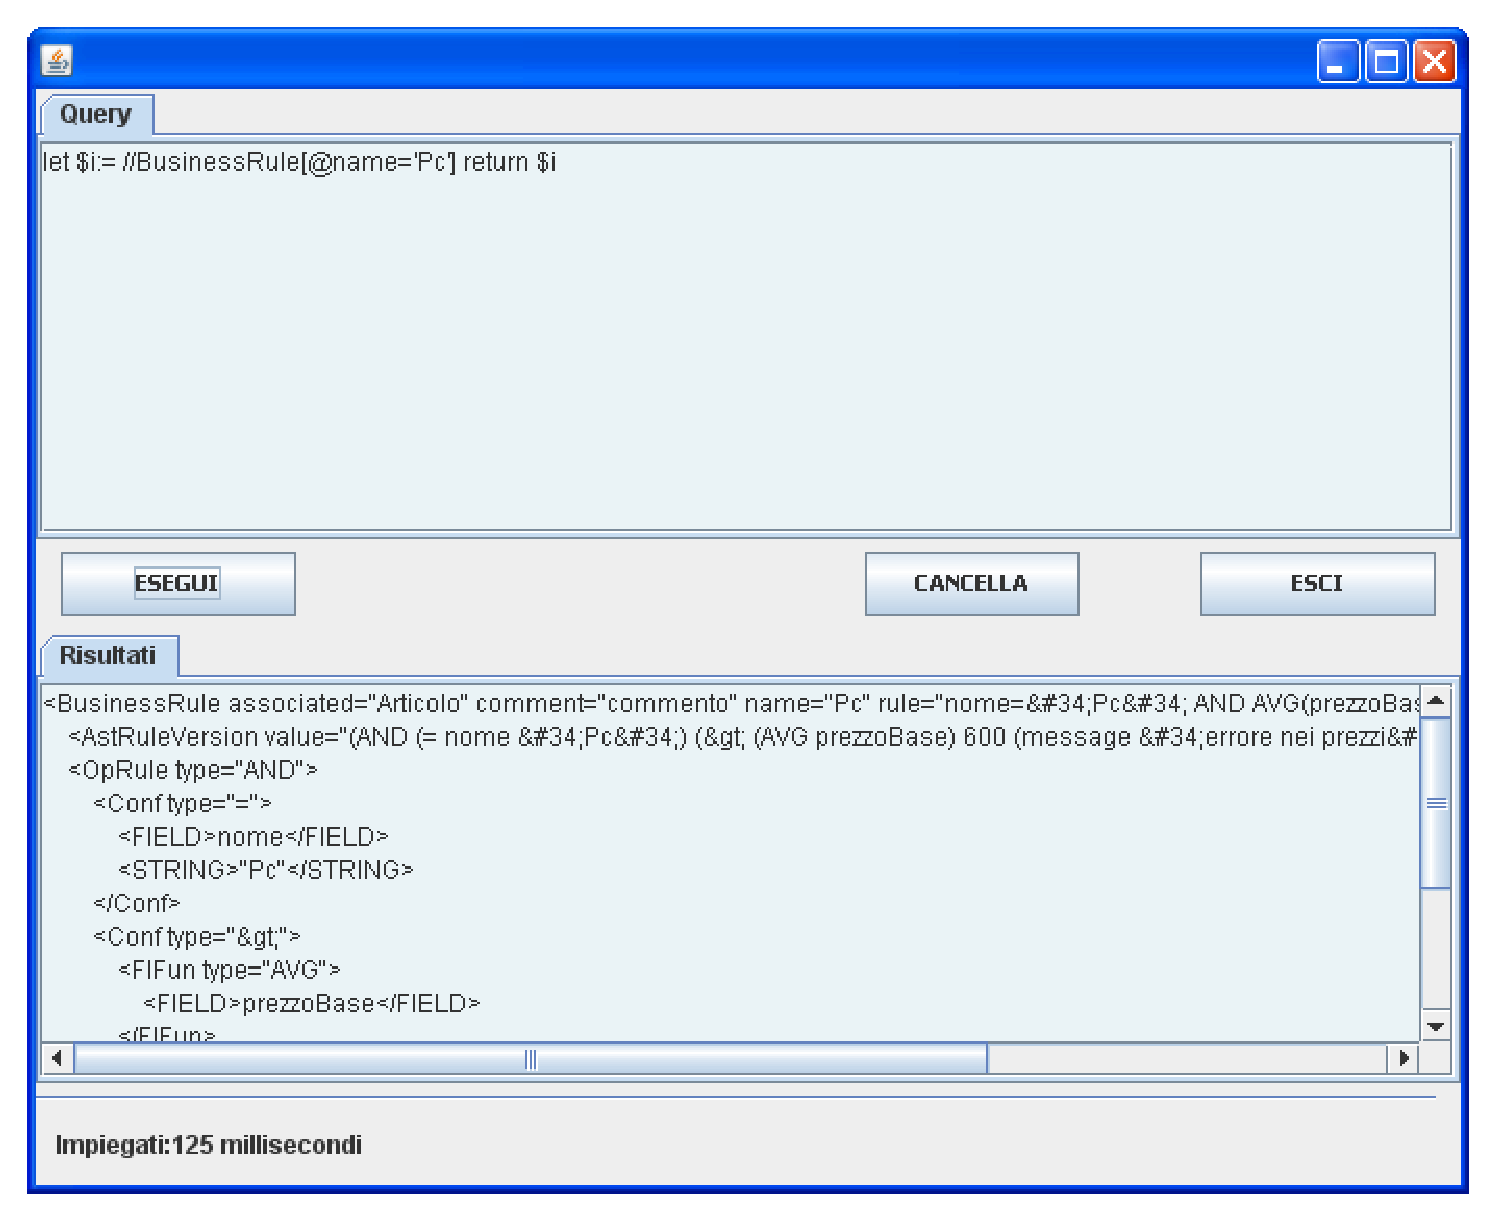
\includegraphics[width=0.7\textwidth]{manuale_utente/sandbox_di_query.eps}\\
 figura 3.4.1 esempio di querying corretta
\end{center}
La figura 3.4.1 mostra l'esito positivo di una query e in particolare verr\`a visualizzato nel campo dati ``Risultati'' l'esito della query e nella barra sottostante il tempo di risposta (in millisecondi) impiegato da \underline{eXist}. 

\begin{center}
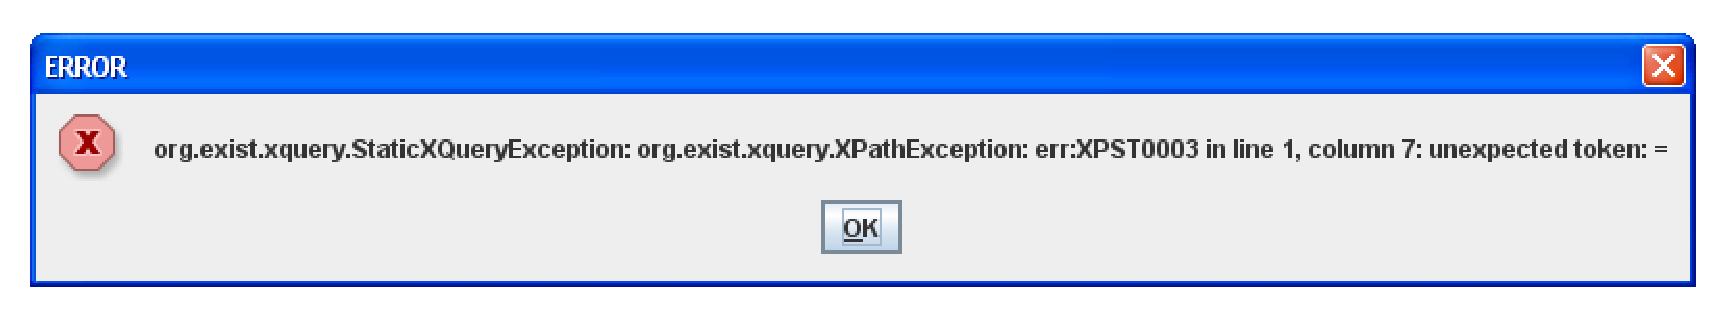
\includegraphics[width=1.1\textwidth]{manuale_utente/esempio_errore_sandbox_query_errata.eps}\\
figura 3.4.2 eccezione di querying errata
\end{center}
La figura 3.4.2 mostra un'eccezione lanciata in caso di esito negativo di una query scritta in maniera errata.

\chapter{Appendice}
\section{Messaggi di errore e loro significato}
\begin{table}[htbp]
\begin{tabular}{||p{6.5cm}||p{6.5cm}||}
\hline
\textbf{Messaggio:} & \textbf{Descrizione:} \\ \hline
Autenticazione fallita! & Nome utente e/o password non inseriti correttamente..\\ \hline
Server eXist spento! & Il server eXist non \`e avviato. \\ \hline
Oggetto associato \textless nome associato\textgreater\ inesistente! & Inserimento di una \underline{business rule} con un business object associato non valido. \\ \hline
Campo dati \textless nome campo dati\textgreater\ non trovato: validazione interrotta! & Riferimento ad un campo dati sbagliato. La validazione viene interrotta. \\ \hline
Operazione non consentita! \textless tipo 1\textgreater\ != \textless tipo 2\textgreater\ : validazione interrotta! & Errore tra tipi. Esecuzione di un'operazione di confronto tra due tipi diversi. La validazione viene interrotta. \\ \hline
Errore sintattico \textless tutta la \underline{business rule} scritta fino all'errore\textgreater\ : validazione interrotta! & Errore di scrittura nella \underline{business rule}. La validazione viene interrotta. \\ \hline
Regola \textless nome regola\textgreater\  gi\`a presente: inserimento fallito! & La regola ha un nome gi\`a presente nel repository. Non verr\`a quindi inserita. \\ \hline
\underline{business rule} non trovata! & La \underline{business rule} cercata non \`e stata trovata nel repository. \\ \hline
\end{tabular} \\
\end{table}


\end{document}
